\documentclass[a4paper,12pt]{mwart}

\usepackage{polski}
\usepackage[utf8]{inputenc}
\usepackage{float}
\usepackage{color}
\usepackage{hyperref}
\usepackage{listings}
\usepackage{tikz}
\usetikzlibrary{positioning,shapes,shadows,arrows}

\lstset{
  basicstyle=\scriptsize
}

\newcommand{\TODO}[1]{\textcolor{blue}{TODO: #1 \\}}
\newcommand{\ang}[1]{ang.~{\itshape #1}}

% http://tex.stackexchange.com/questions/83440/inputenc-error-unicode-char-u8-not-set-up-for-use-with-latex
\DeclareUnicodeCharacter{00A0}{~}

\begin{document}

\title{Predicting Jams\\%
{\large czyli model prognozujący tworzenie się korków samochodowych} }

\author{Łukasz Jędrzejewski \and Artur Sawicki}

\maketitle

\section{Opis projektu}
W ramach projektu realizowaliśmy zadanie polegające na zbudowaniu modelu prognozującego tworzenie się korków na podstawie historychnych obserwacji. Zadanie opiera się na zadaniu ze strony \href{http://tunedit.org/challenge/IEEE-ICDM-2010/jams}{tunedit.org}.

Do realizacji celów zadania użyliśmy bazy danych \href{https://www.postgresql.org/}{PostgreSQL} rozszerzonej o dodatek umożliwiający pracę z danymi przestrzennymi \href{http://postgis.net/}{PostGIS}. Aby ułatwić pracę na różnych maszynach, baza danych wraz z rozszerzeniem zainstalowana jest na kontenerze typu \href{https://www.docker.com/}{docker}. Skrypty odpowiadające za stworzenie schematu w bazie danych, przetwarzanie i wizualizację danych oraz właściwe obliczenia napisaliśmy w języku \href{https://www.python.org/}{python}.

\section{Opis problemu}
\subsection{Wprowadzenie}
Stacje radiowe wpadły na pomysł zbierania informacji dotyczących zatłoczenia ulic oraz przekazywanie ich do kierowców, w celu umożliwienia im omijania nieprzejezdnych dróg. Takie dane można użyć też w inny sposób - na ich podstawie można przewidzieć, gdzie mogą pojawić się kolejne korki, bazując na początkowym stopniu zatłoczenia ulic. Tego właśnie dotyczy zadanie.

\subsection{Dane}
Dane użyte w zadaniu wygenerowane zostały z jedno-godzinnych symulacji. Każda z nich zaczynała się prawie pustą siecią dróg, do której dodawane są samochody, z losowo wybranym punktem startu i docelowym.

Na początku każdej symulacji 5 losowych odcinków dróg (2 główne i 3 mniejsze) zostawało usuniętych z grafu imitując roboty drogowe. Jako dane wejściowe algorytm dostaje identyfikatory 5 usuniętych dróg oraz sekwencję identyfikatorów dróg, na których korek pojawił się w ciągu pierwszych 20 minut symulacji. Zadaniem jest przewidzenie korków w następnych 40 minutach.

Odcinek uznajemy za zakorkowany kiedy średnia prędkość w ciągu ostatnich 6 minut nie przekroczyła 5km/h, a liczba samochodów jaka przejchała lub znajduje się na nim jest większa niż 10.

Zbiór treningowy i zbiór testowy zawierają po 5000 próbek, z których każda jest pojedynczą symulacją. Dane treningowe zawierają pierwsze 20 minut symulacji oraz kolejne 40 minut, natomiast dane testowe - tylko pierwsze 20 minut.

Dostępny jest także graf ulic.

Na~koniec należy wspomnieć, że~zgromadzone dane dotyczą Warszawy.

\subsection{Wizualizacja}
Powyższe dane zwizualizowaliśmy. Nie miało to wpływu na predykcję, jednak pozwoliło nam obejrzeć dane, z którymi pracowaliśmy. Poniżej prezentujemy efekty.

\begin{figure}[h]
\centerline{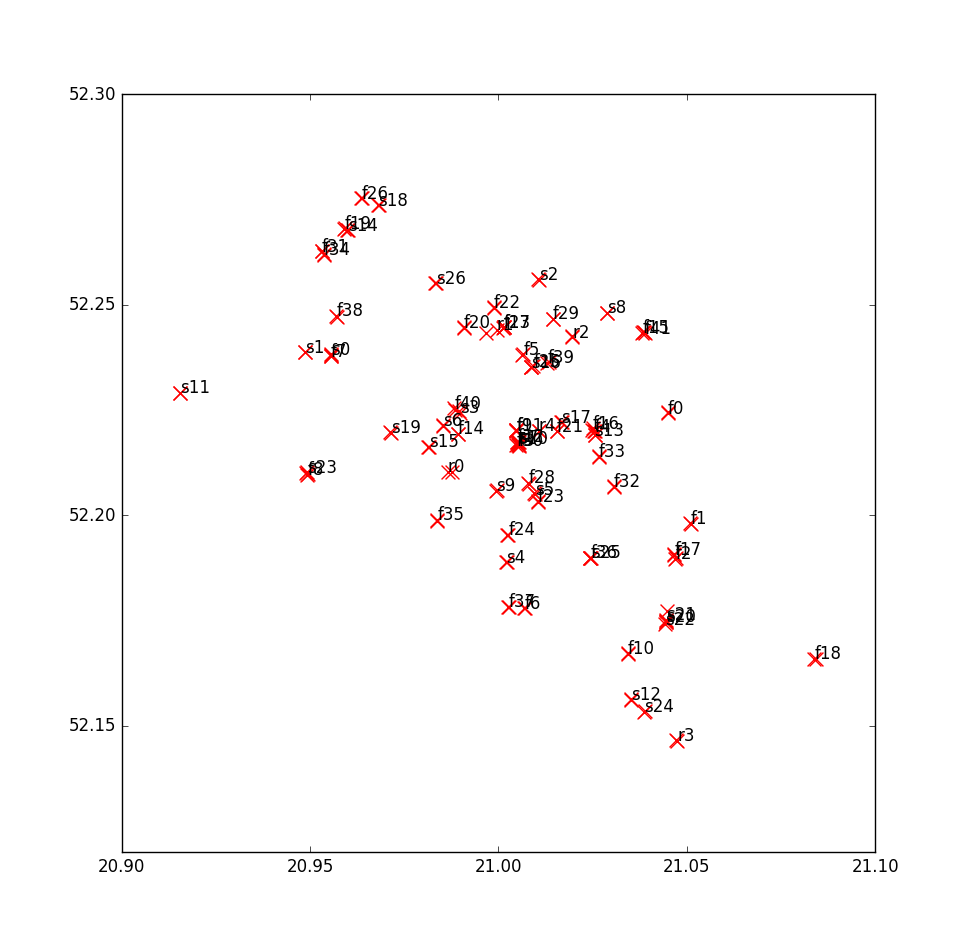
\includegraphics[width=\textwidth]{figures/jams.png}}
\caption{Rysunek przedstawia wszystkie korki znajdujące się w danych treningowych. Litera f oznacza korek z pierwszych 20 minut, litera s - z~kolejnych 40. Numery wyznaczają kolejność korków.}
\end{figure}

\begin{figure}[h]
\centerline{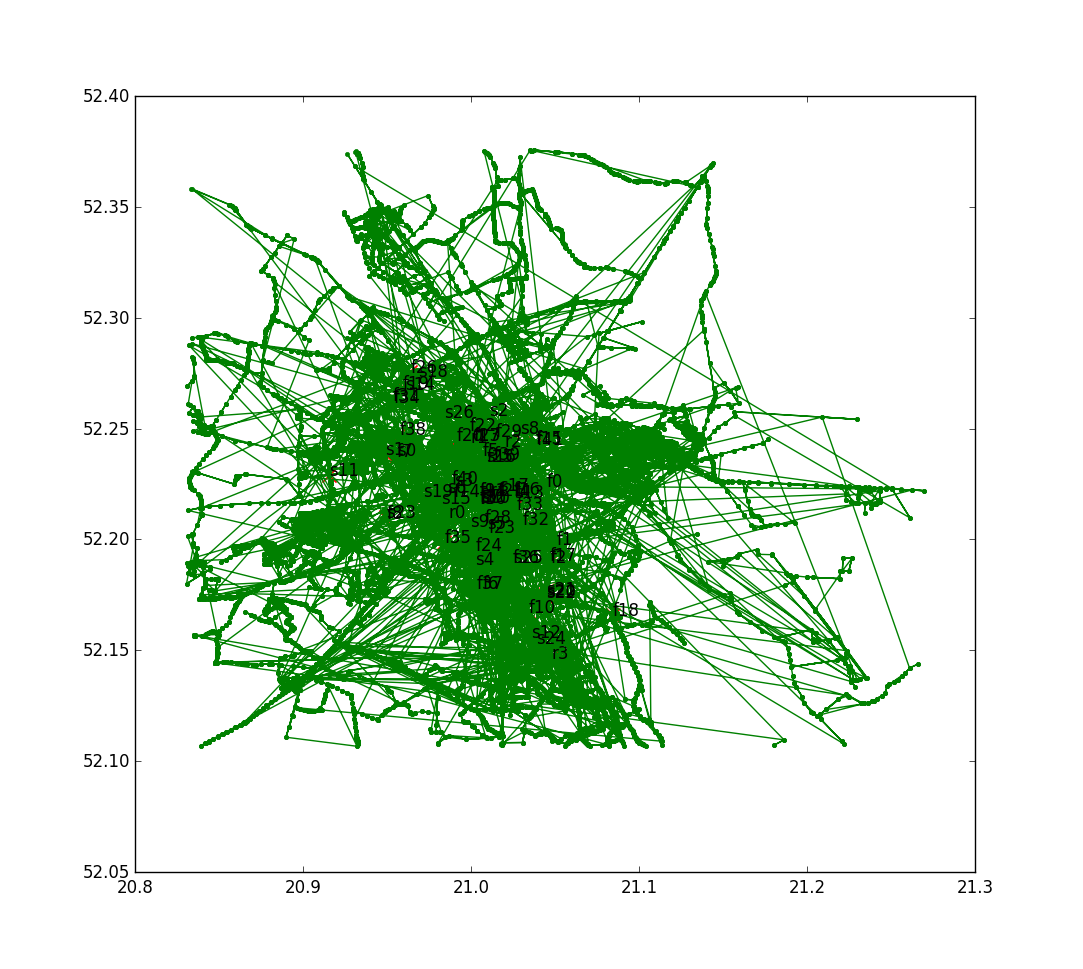
\includegraphics[width=\textwidth]{figures/map.png}}
\caption{Rysunek pokazuje wszystkie drogi zawarte w grafie.}
\end{figure}

\section{Model danych}

\begin{figure}[H]
\centerline{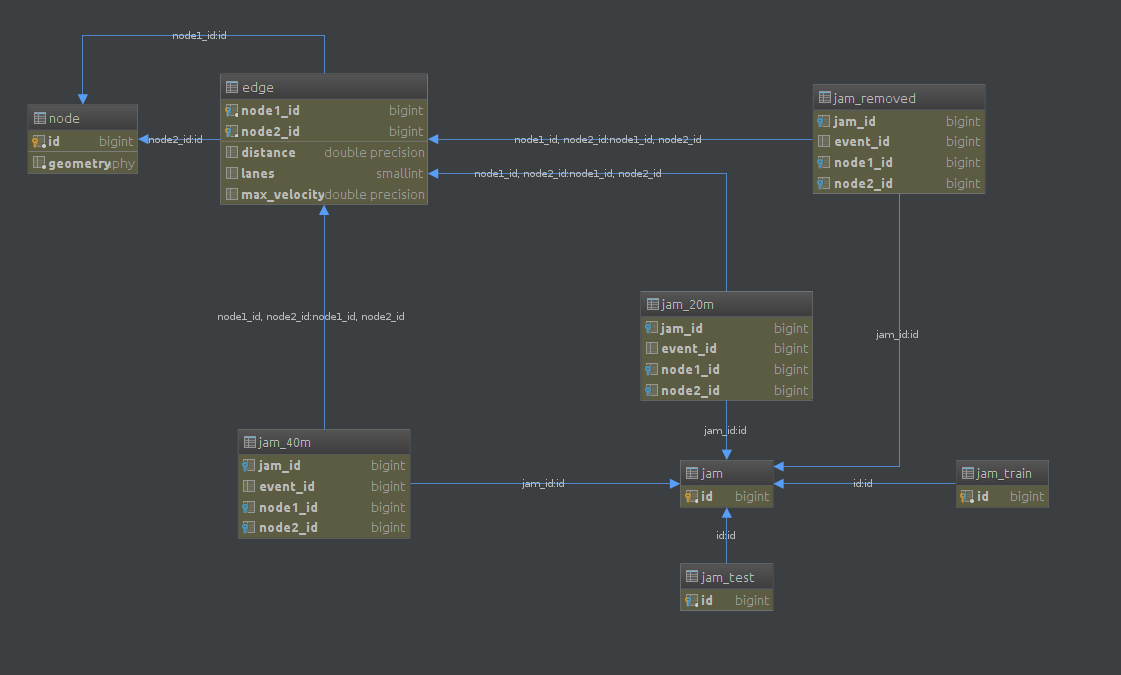
\includegraphics[width=\textwidth]{figures/diagram.png}}
\caption{Model danych zaprezentowany na diagramie relacji.}
\end{figure}

\section{Predykcja}

\subsection{Dane}

Udostępniony zbiór treningowy zawierających 5000 symulacji podzieliśmy na~dwa zbiór treningowy składający się z~4500 symulacji oraz zbiór testowy zawierających 500 przykładów. Nie zdecydowaliśmy się skorzystać z~zamieszczonego na~stronie zadania zbioru testowego, ponieważ zawierał on~tylko dane z~20 pierwszych minut. W~związku z~tym do~oceny zbudowanego modelu używamy części danych treningowych.

\subsection{Ocena rozwiązania}

Do~oceny poprawności predykcji korków w~ciągu kolejnych 40~minut, wykorzystaliśmy miarę zaproponowaną przez pomysłodawców zadania. Została ona użyta do~oceny rozwiązań zgłoszonych w~trakcie trwania konkursu w~2010 roku.

Poniżej zamieściliśmy oryginalną formułę do~porównywania podobieństwa dwóch rozwiązań:

\[quality(P, T) = \frac{1}{N}\sum_{i = 1}^N Precision(P, T, i)\]

\[Precision(P, T, i) = \frac{\left | P_i \cap T_i \right |}{i}\]

\[N = \max (\left | P \right |, \left | T \right |)\]

gdzie:

\begin{itemize}
\item $P$, $T$ -- listy zawierające segmenty kolejno zakorkowanych dróg w~ciągu 40 minut,
\item $P_i$, $T_i$ -- zakorkowany segment drogi na~pozycji $i$ rozwiązania,
\item $\left | P \right |$, $\left | T \right |$ -- liczba zakorkowanych segmentów w~ciągu 40 minut.
\end{itemize}

Tak zdefiniowana formuła oceny posiada kilka cech. Najważniejszą wydaje się mocniejsze premiowanie poprawnych predykcji na~początku listy segmentów. W~szczególności, pierwszy segment będzie ma~wpływ na~ocenę wszystkich kolejnych segmentów -- zarówno w~ujęciu pozytywnym, jak i~negatywnym. Kolejną cechą jest uwzględnianie kolejności, zatem rozwiązania zawierające wszystkie dokładnie wszystkie segmenty jak rozwiązanie wzorcowe, nie otrzymają wzorcowej oceny.

\subsection{Algorytm}

\subsection{Wyniki}

\section{Uruchamianie}
\subsection{Baza danych}
Aby uruchomić bazę danych należy:
\begin{enumerate}
\item Zainstalować program docker dostępny na stronie \href{https://www.docker.com/}{docker.com}.
\item Uruchomić kontener zawierający bazę PostgreSQL z rozszerzeniem PostGIS:
\begin{lstlisting}
sudo docker run --name "postgis" -p 25432:5432 -d -t kartoza/postgis
\end{lstlisting}
\item Połączyć się z bazą używając polecenia psql:
\begin{lstlisting}
psql -h localhost -U docker -p 25432 -d postgres
\end{lstlisting}
\item Włączyć dodatek:
\begin{lstlisting}
create extension Postgis;
\end{lstlisting}
\item Stworzyć bazę danych:
\begin{lstlisting}
create database "predicting-jams" owner docker encoding 'UTF8' template template_postgis;
\end{lstlisting}
\item Przełączyć się na utworzoną bazę danych:
\begin{lstlisting}
\c "predicting-jams"
\end{lstlisting}
\item Stworzyć schemat (zakładamy połączenie z bazą przez psql z głównego katalogu projektu):
\begin{lstlisting}
\i sql/create.sql
\end{lstlisting}
\item (opcjonalnie) Jeżeli będzie potrzeba zrzucenia schematu:
\begin{lstlisting}
\i sql/drop.sql
\end{lstlisting}
\end{enumerate}

\subsection{Wczytywanie danych}
Aby wczytać dane należy uruchomić bazę danych, a następnie wykonać skrypt:
\begin{lstlisting}
python3 load_data.py
\end{lstlisting}

\subsection{Wizualizacja danych}
Aby zwizualizować dane należy wykonać skrypt:
\begin{lstlisting}
python3 visualize.py
\end{lstlisting}

\subsection{Predykcja}
Aby dokonać predykcji:
\begin{lstlisting}
python3 predict.py
\end{lstlisting}

\section{Podsumowanie}
Ale fajno...

\end{document}
